\section{Signal signature and base selection}

To build an effective analysis strategy, the signal kinematics must be studied and exploited. The electroweakino production in question exhibit unique features which can be used in order to discriminate between the signal and the \gls{sm} background. It is important to explore these signal distributions in order to define a preselection, or a base cut, that will serve the purpose of retaining as much signal as possible while rejecting as much background. All of the following distributions were plotted by weighting the simulation to Run II luminosity of $\lumi = 135 \fbinv$ and requiring at least one jet in the event with $\pt \geq 30\GeV$. Further selection might apply and will be listed in each section in that case.

\subsection{Missing Transverse Energy}
\label{subsec:signal-met-mht}
One property that essentially all \gls{dm} searches have in common is the presence of a \gls{dm} candidate in the production. The exact identity and properties of said particle (or particles in the case multiple \gls{dm}  candidates) vary, but they do share a lot in common. The \gls{dm} candidate in our \gls{susy} search is the \gls{neutralino}, which is a type of \gls{dm} candidate referred to as a \gls{wimp}. A \gls{wimp}, broadly speaking, is a new elementary particle which interacts via gravity and any other force (or forces), potentially not part of the \gls{sm} itself, which is as weak as or weaker than the weak nuclear force, but also non-vanishing in its strength. That essentially means that such candidate is neutral, and therefore not interacting via the electromagnetic force. A neutral particle that interacts neither electromagnetically nor via the strong force (\ie colorless) will escape detection and will leave traces in the form of a transverse momentum imbalance, which we refer to as \gls{met} (Missing Transverse Energy or Missing Transverse Momentum). Our signal contains two \gls{dm} candidates in the production, which are the \glspl{lsp}, the \glspl{neutralino} \neuto. We therefore expect the signal to contain considerable magnitude of \gls{met}. As described in~\ref{subsec:met}, \fxnote{make sure we described both met and mht} we are more interesting in \gls{mht}, which is highly correlated with \gls{met}, due to our definition of lepton isolation and its use in the background estimation methods. Nonetheless, we will look at both $\MET$ and $\mht$ observables.
\fxnote{make sure we define the different deltaM somewhere}
\begin{figure}[h]
\centering
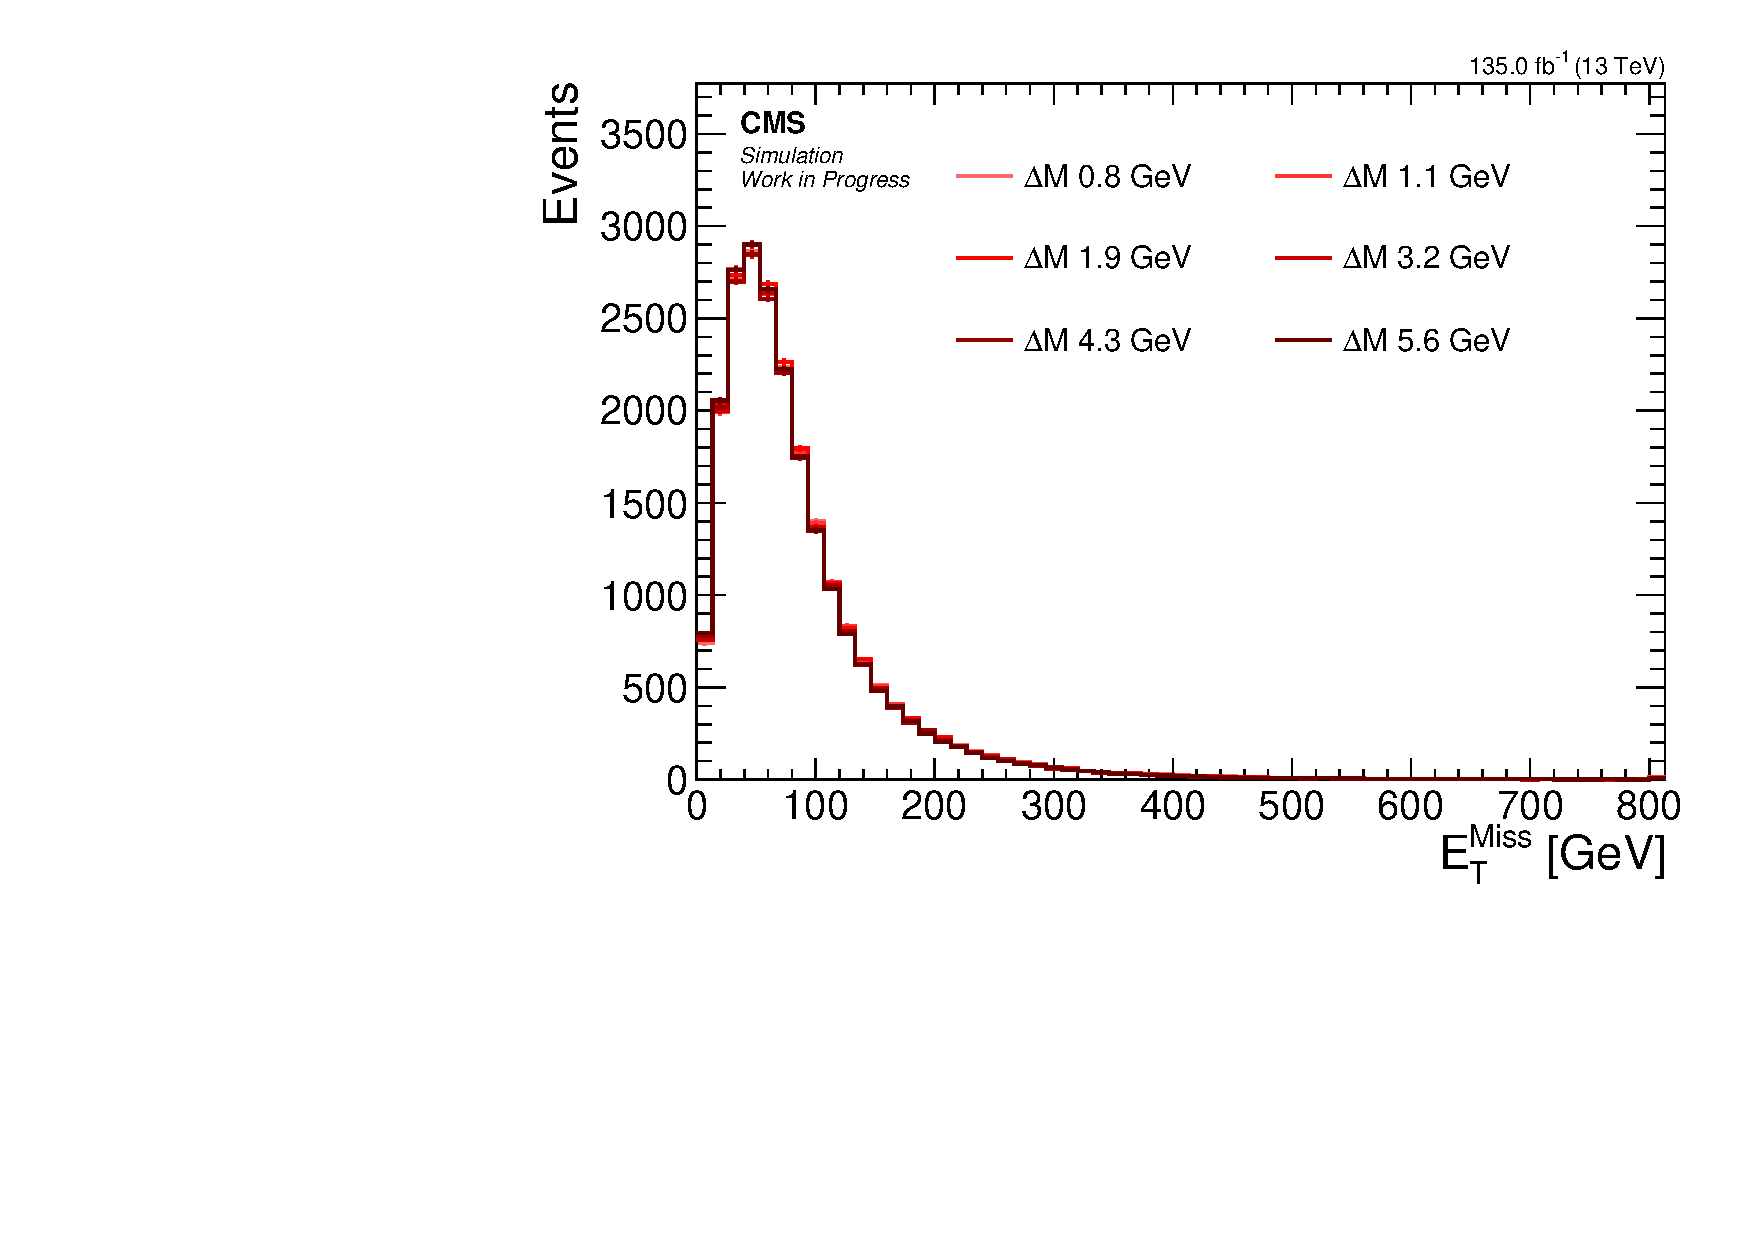
\includegraphics[width=0.48\linewidth]{plots/signal_common_distributions_fixed_mu/none_MET.pdf} \,
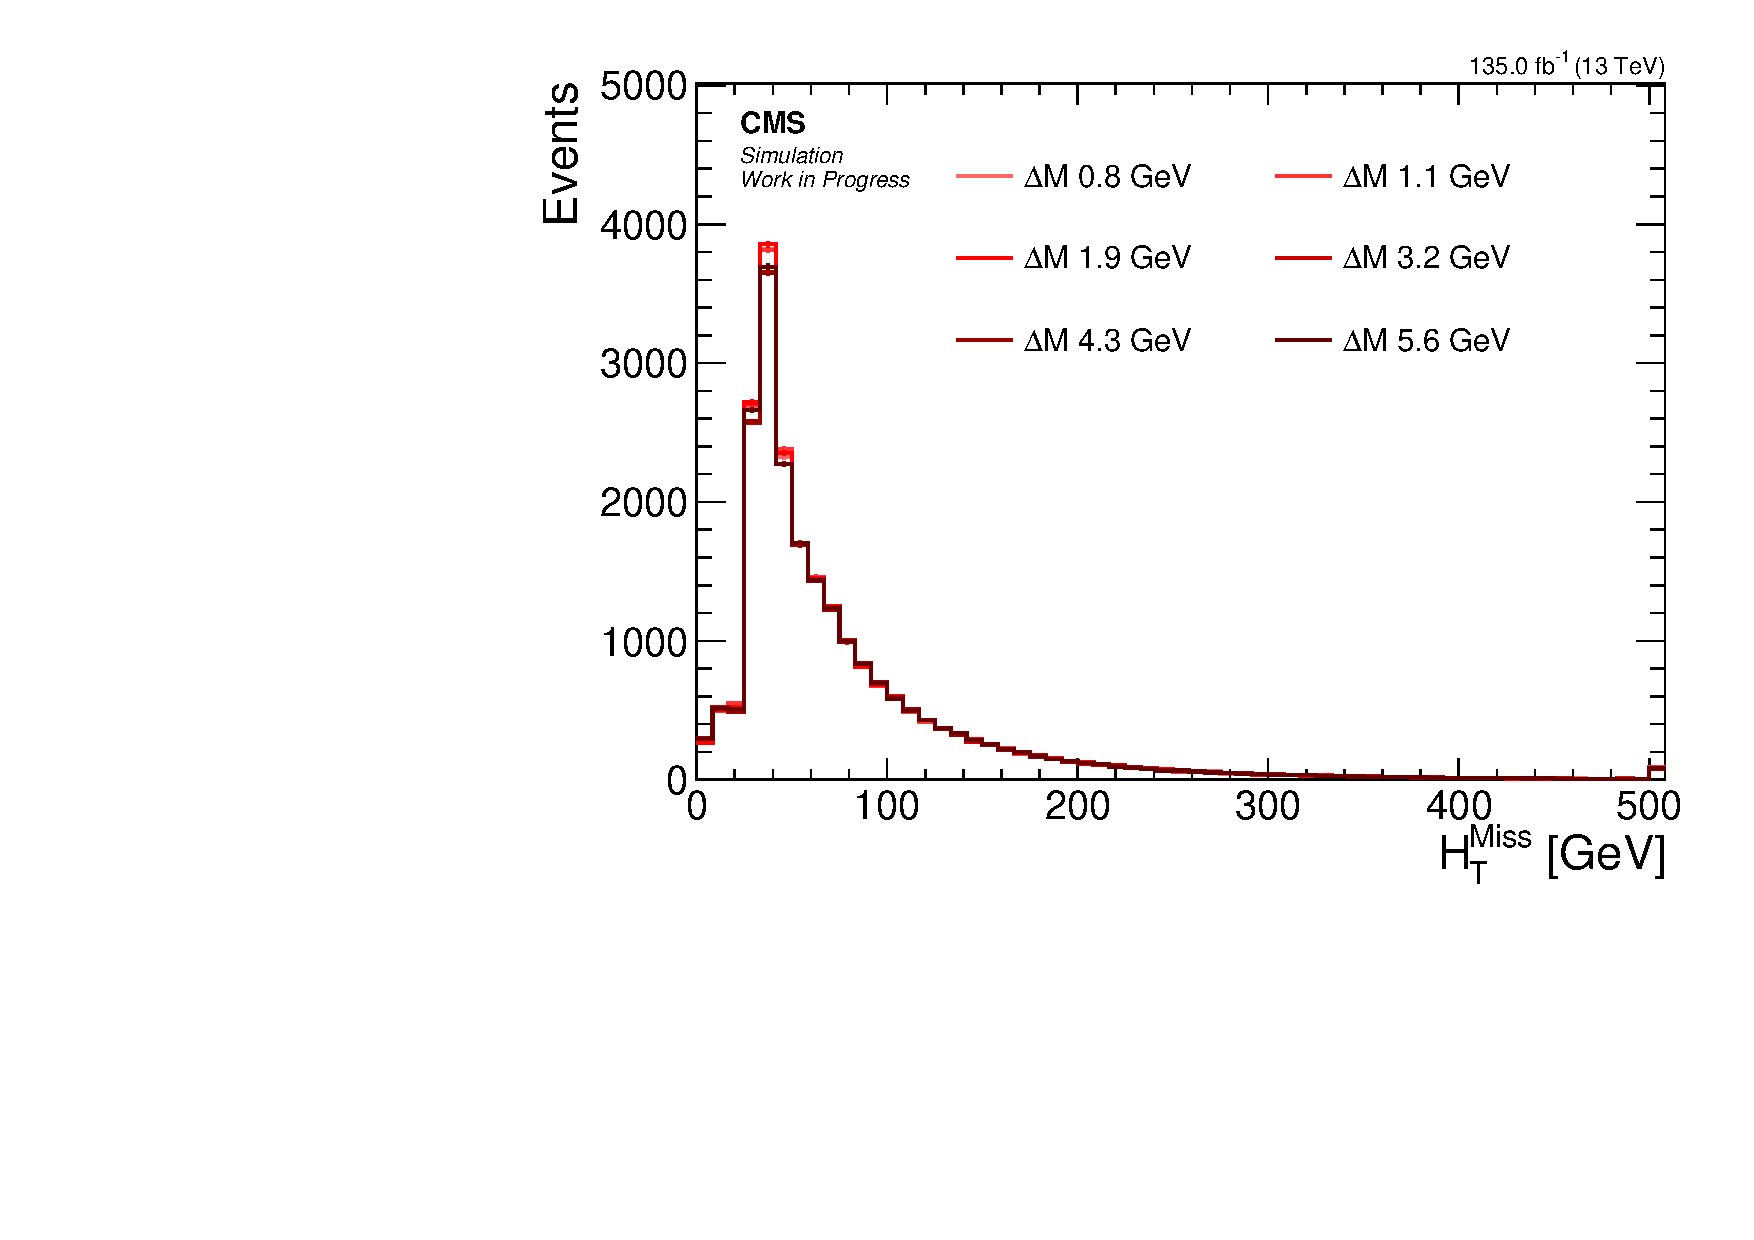
\includegraphics[width=0.48\linewidth]{plots/signal_common_distributions_fixed_mu/none_MHT.pdf}  \\
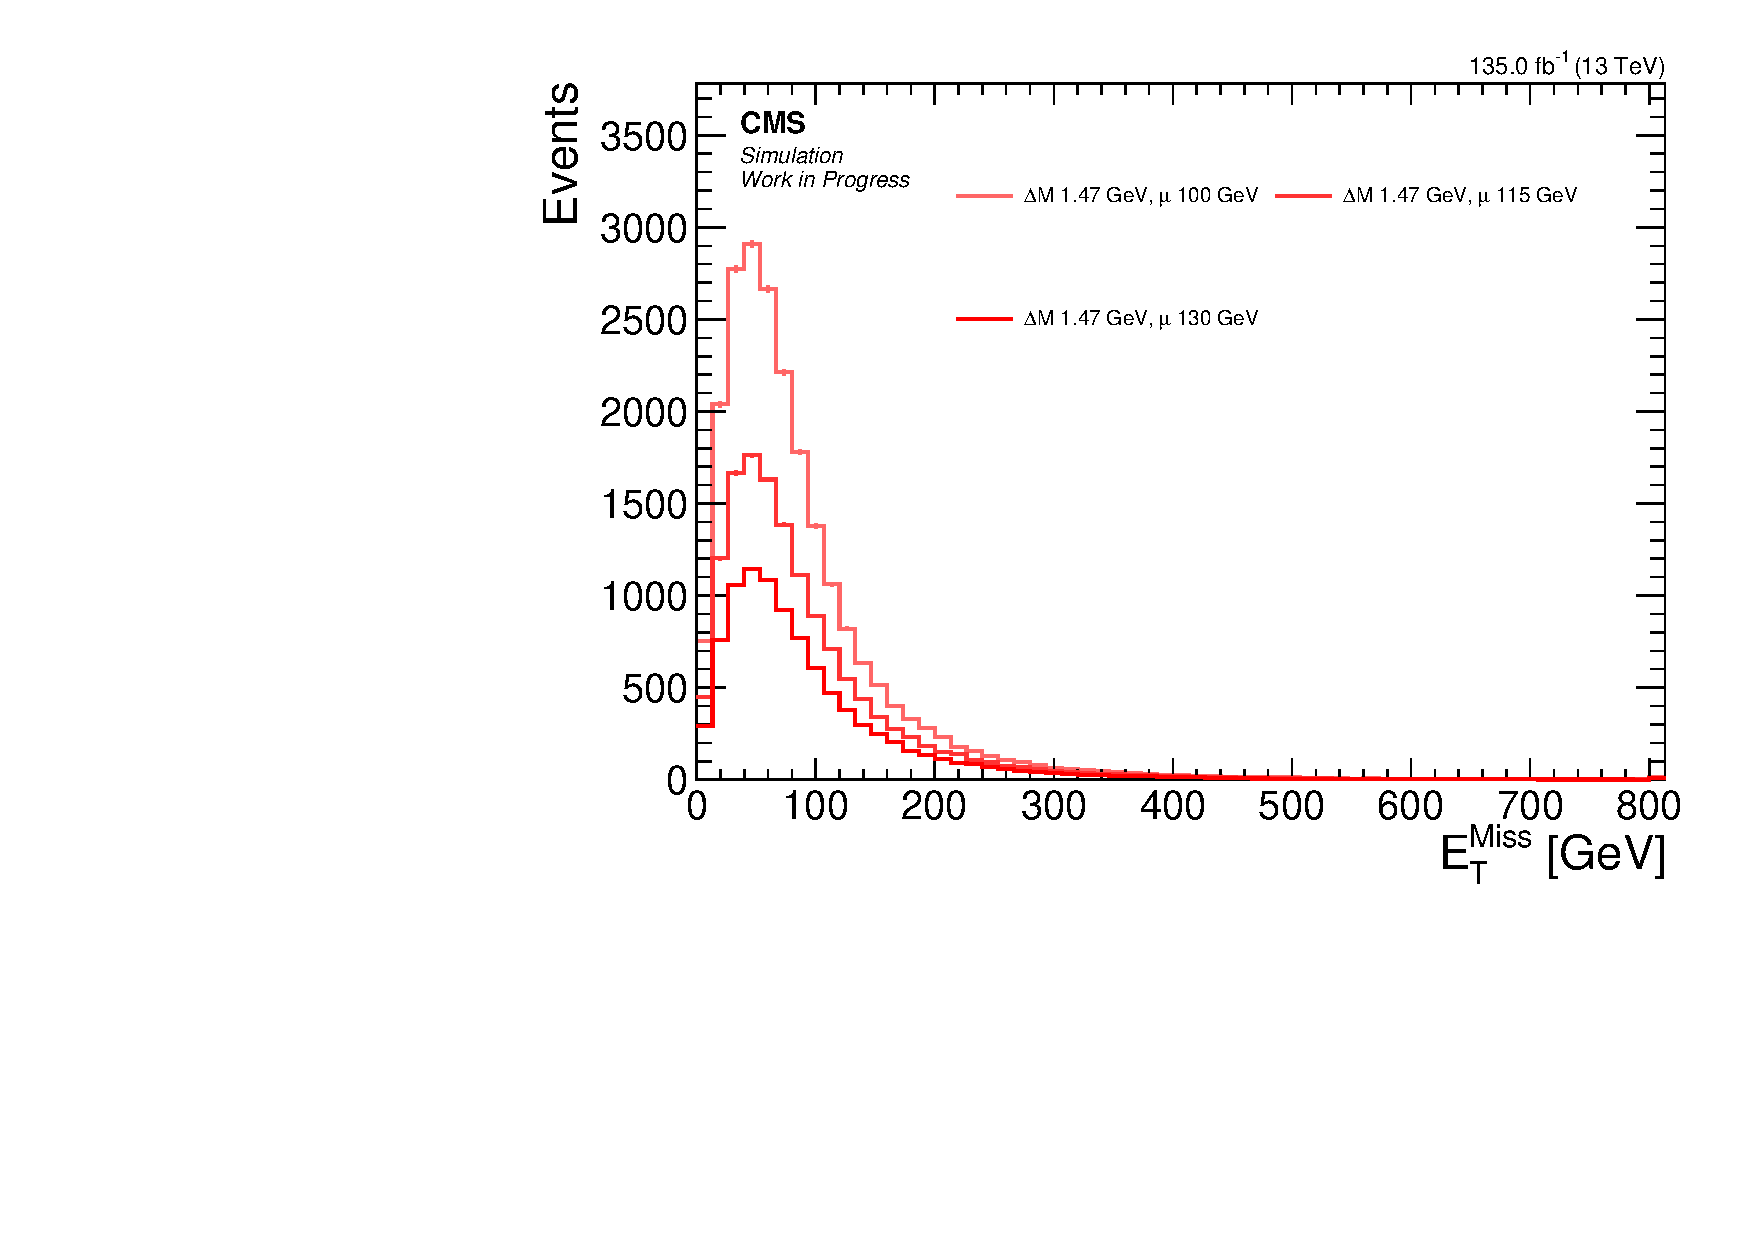
\includegraphics[width=0.48\linewidth]{plots/signal_common_distributions_fixed_dm/none_MET.pdf} \,
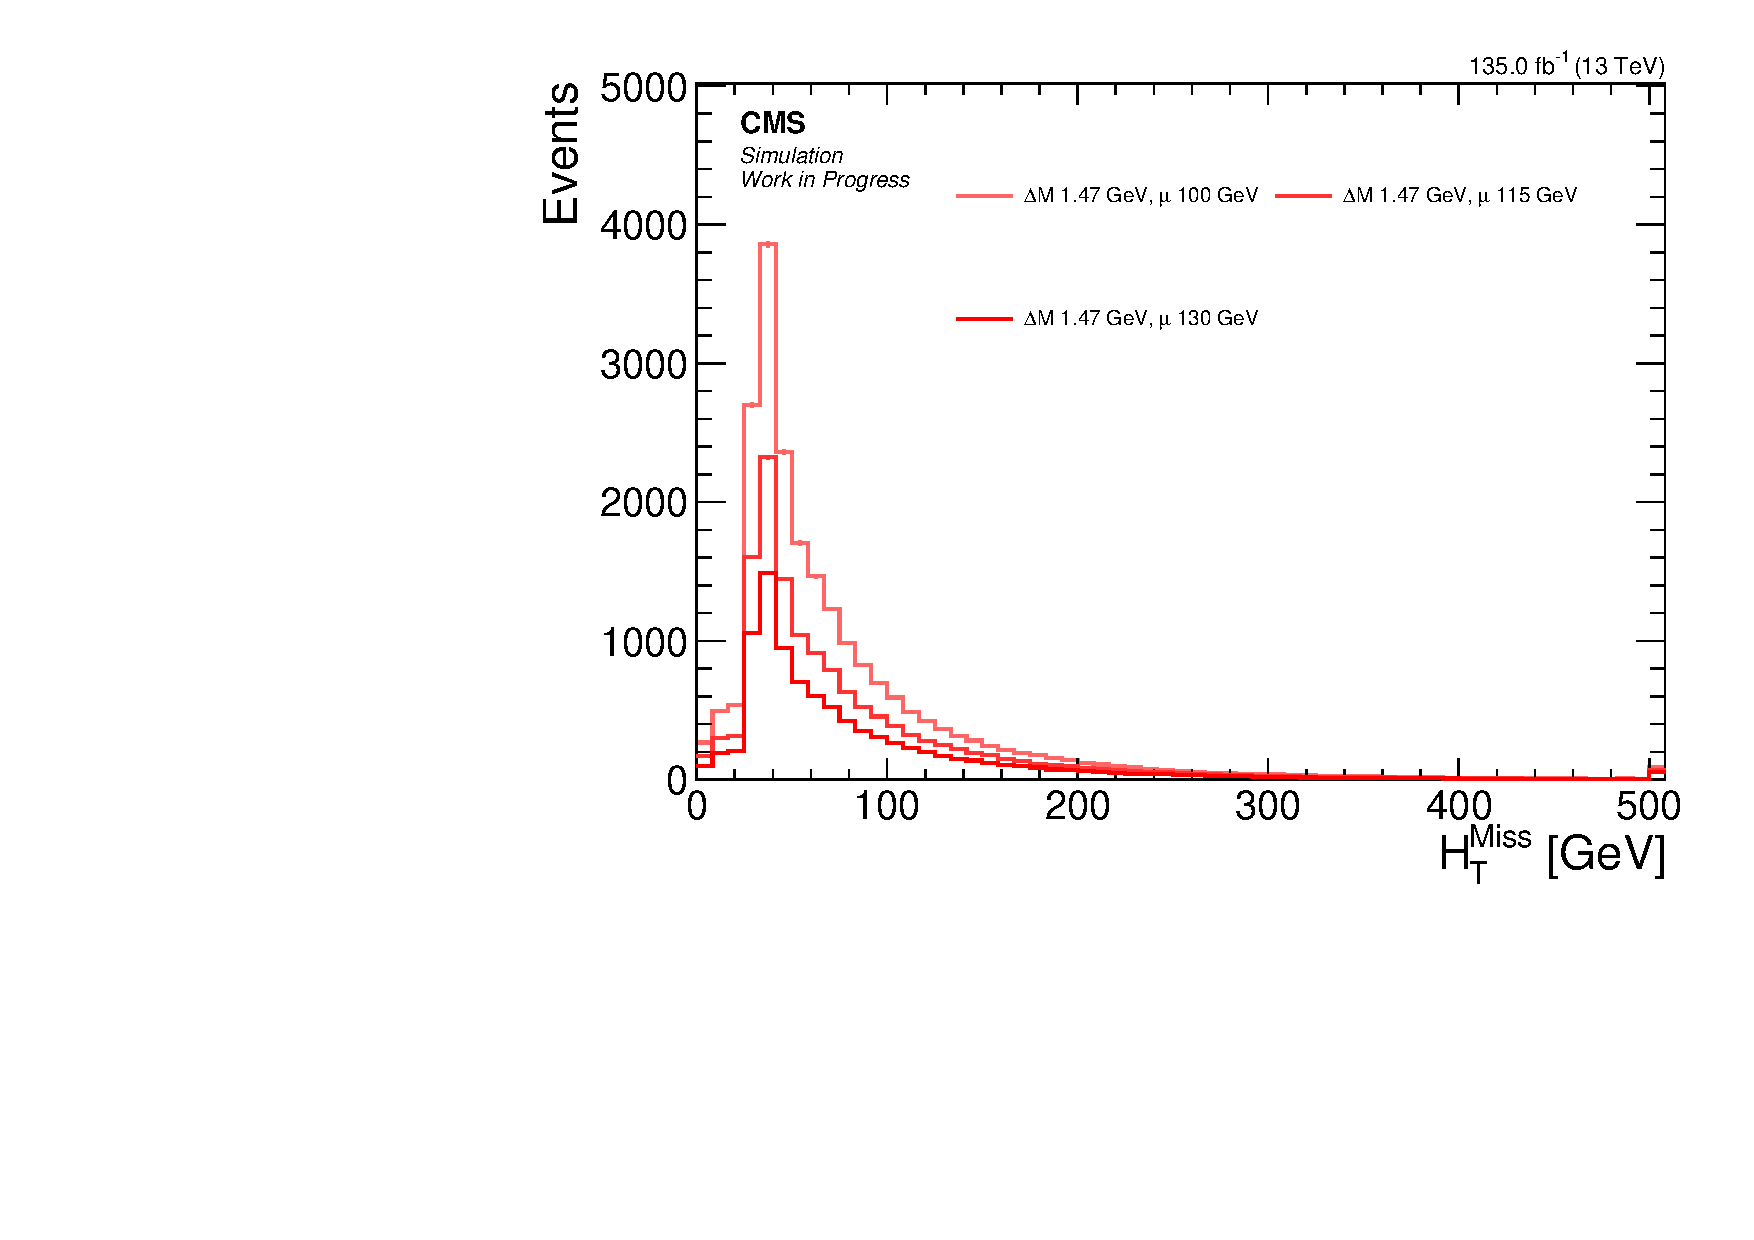
\includegraphics[width=0.48\linewidth]{plots/signal_common_distributions_fixed_dm/none_MHT.pdf}  \\
\caption[Signal $\MET$ and $\mht$ distributions]{ Signal distributions for \MET (left) and \mht (right) comparing various $\dm$ with a fixed higgsino parameter $\mu=100\GeV$ (upper), and comparing various higgsino parameters $\mu$ with fixed $\dm=1.47\GeV$ (lower).}
\label{fig:signal-met-mht}
\end{figure}

As we expect, $\MET$ and $\mht$ are hardly affected by the different choices for \dm, while the higgsino parameter $\mu$ affect the distributions above all through its lower production cross section for higher higgsino parameter $\mu$. As discuss at~\ref{sec:trigger}, the region of interest lie at $\mht\geq 220$ for triggering purposes. Even though this is quite a harsh and inefficient cut, one must look also at the \gls{sm} background at the regions of $\mht < 220$ and $\mht\geq 220$ to conclude that most of the sensitivity comes from the $\mht\geq 220$ region, since the production of real \gls{mht} (or \gls{met}) result from the production of neutrinos in the event, and these are much less common than \gls{qcd} events which swarm the $\mht < 220$ region. Therefore, cutting at $\mht\geq 220$ might be inefficient, but results in high sensitivity. 

\subsection{Jets and hardronic activity}

Since the \glspl{neutralino} \neuto escaping the detector are the contributors to the \gls{mht} and in doing so the drivers of the sensitivity in high \gls{mht} region, we want them to be as boosted as possible, \ie, with the highest transverse momentum \gls{pt} as possible. A widely used approach is to require \fxnote{add citation} an \gls{isr} jet in the event. An \gls{isr} jet is formed when one of the incoming protons emit radiation (such as a photon or a gluon) before the interaction \fxnote{add citation and maybe reference to other section}. If a jet with high enough \gls{pt} is emitted, the rest of the interaction is recoiled against this jet and boosting it in the other direction. This way, the boosted \glspl{neutralino} \neuto will result in higher \gls{mht}. As described in \fxnote{ref}, we require the jets to have $\pt \geq 30\GeV$ and be located within the tracker acceptance $\left(\abs{\eta}<2.4\right)$. We require at least one such jet in the event.
\begin{figure}[h]
\centering
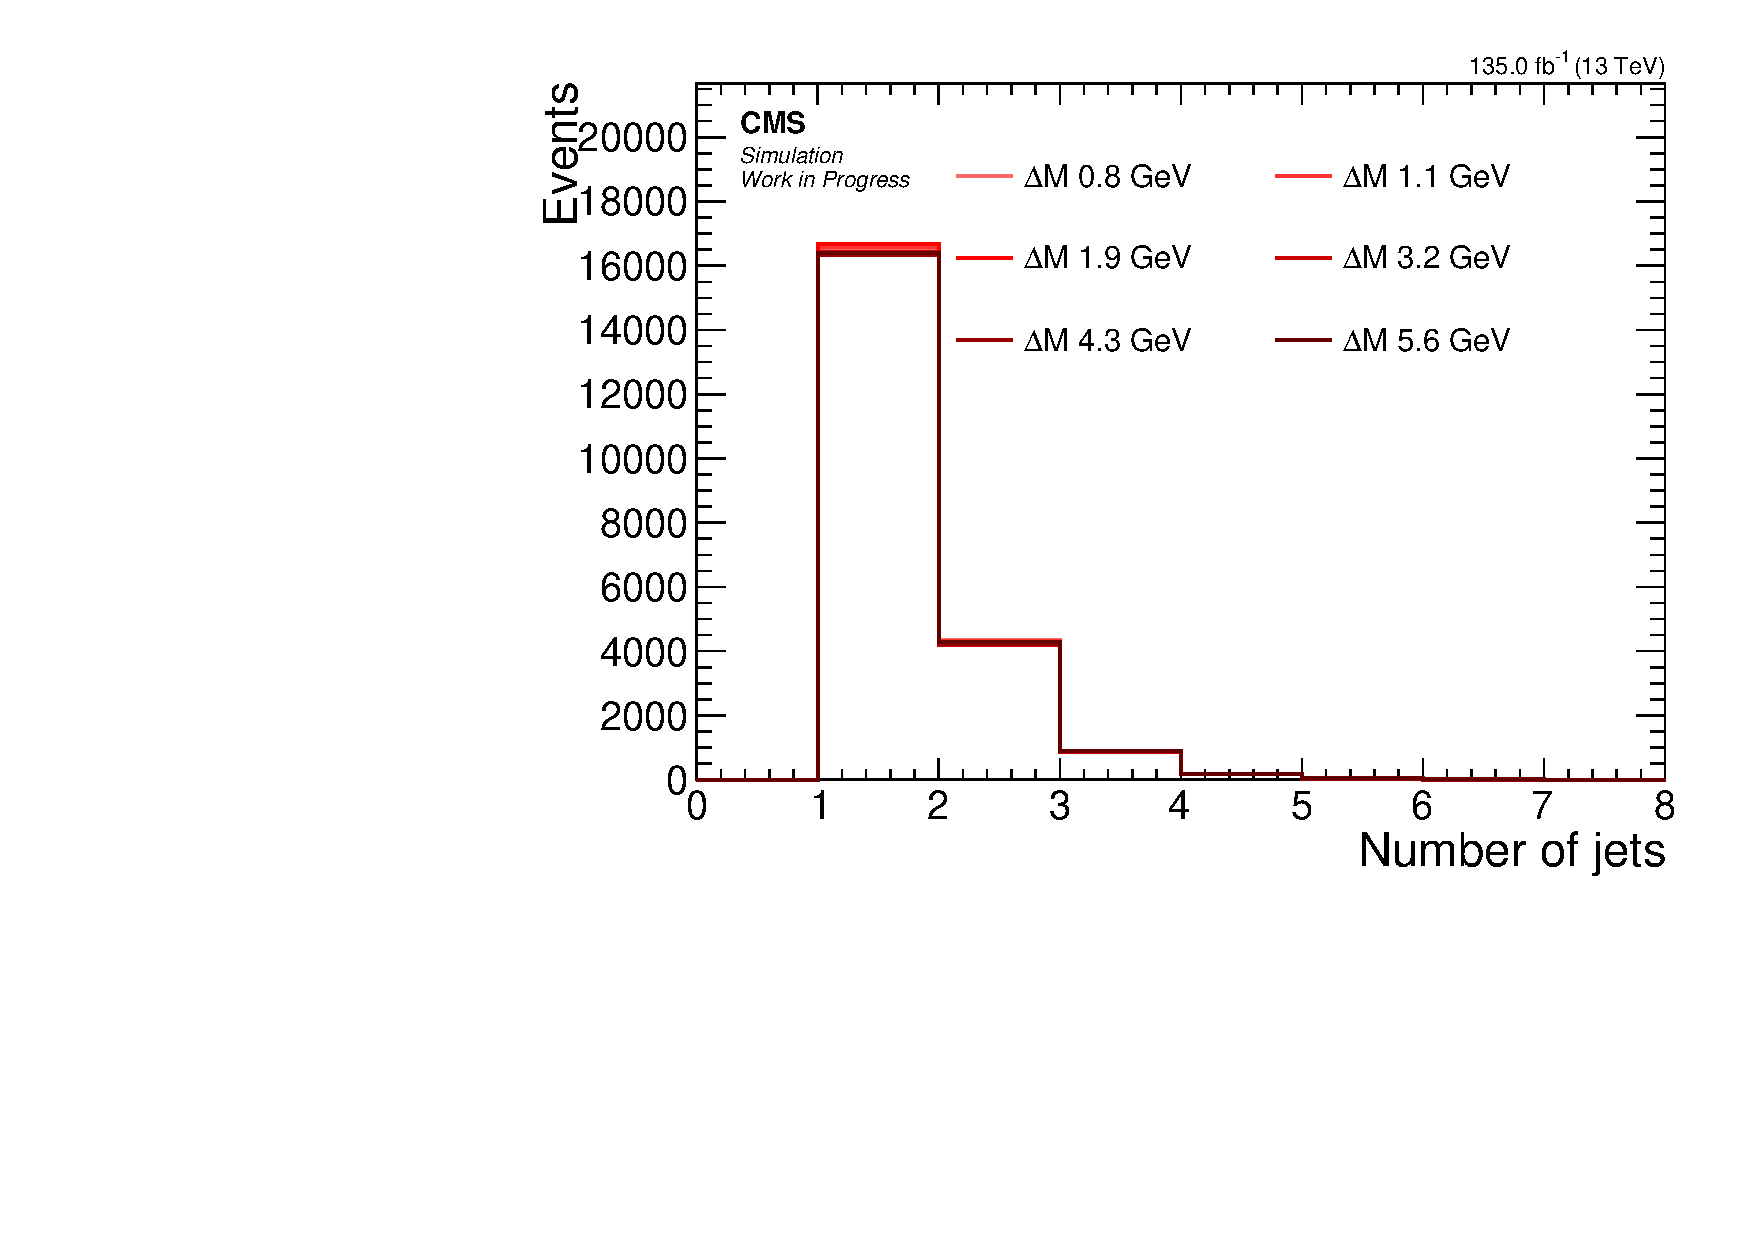
\includegraphics[width=0.48\linewidth]{plots/signal_common_distributions_fixed_mu/none_NJets.pdf} \,
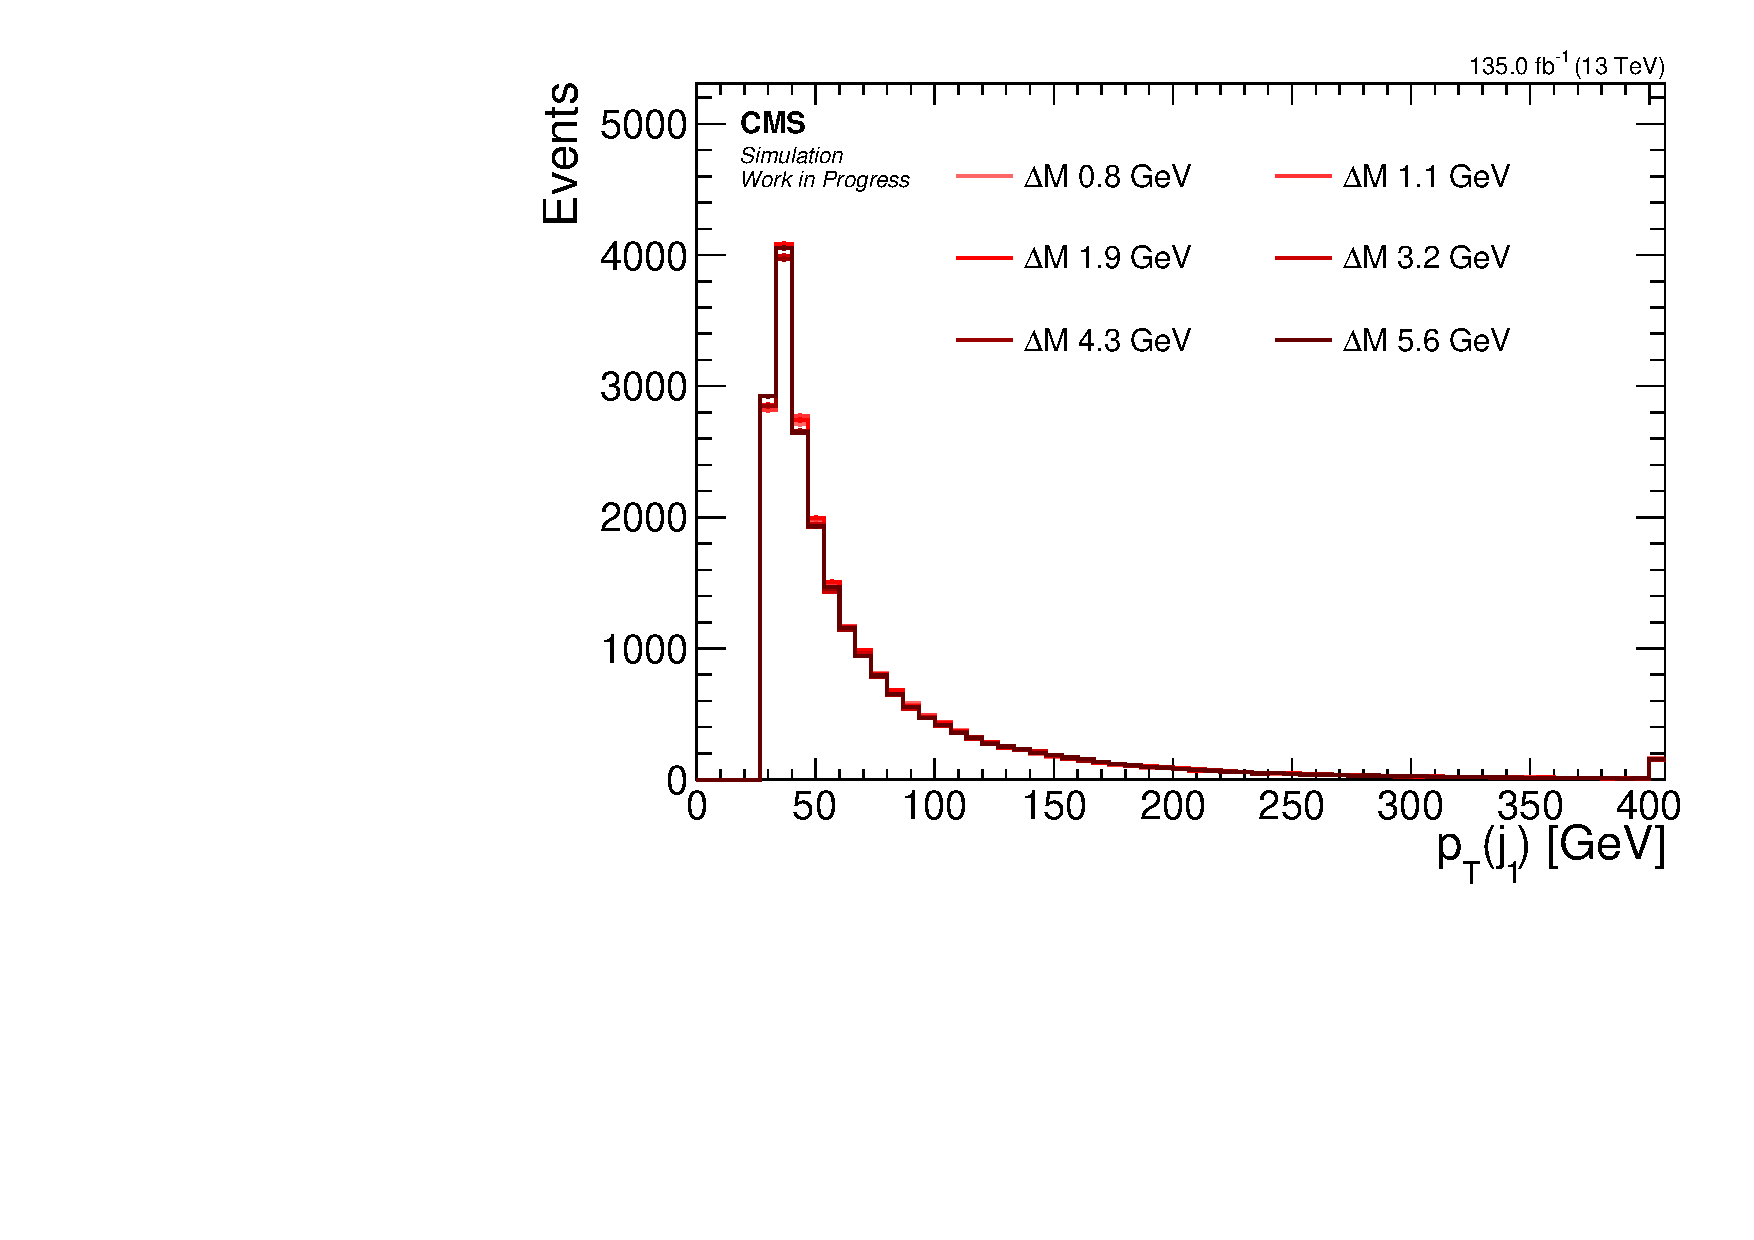
\includegraphics[width=0.48\linewidth]{plots/signal_common_distributions_fixed_mu/none_LeadingJetPt.pdf}  \\
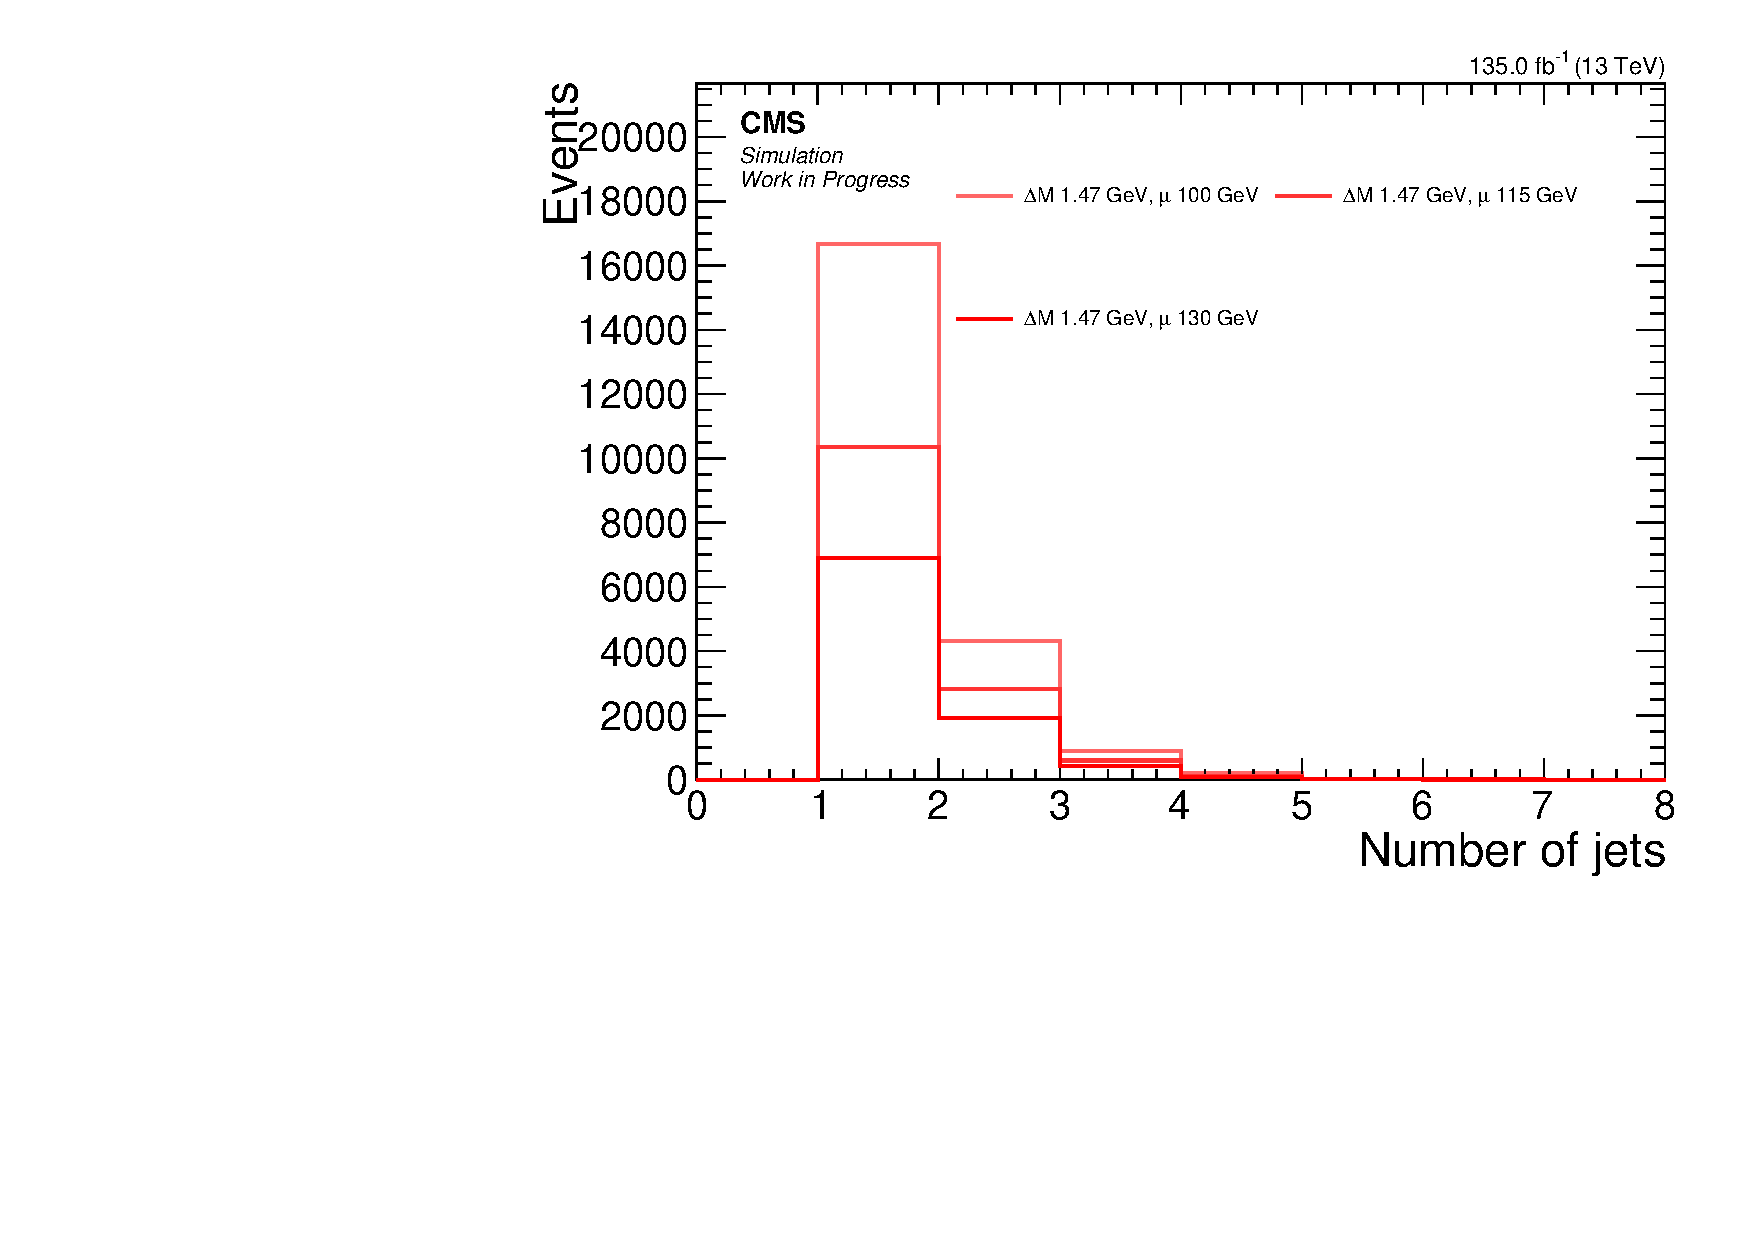
\includegraphics[width=0.48\linewidth]{plots/signal_common_distributions_fixed_dm/none_NJets.pdf} \,
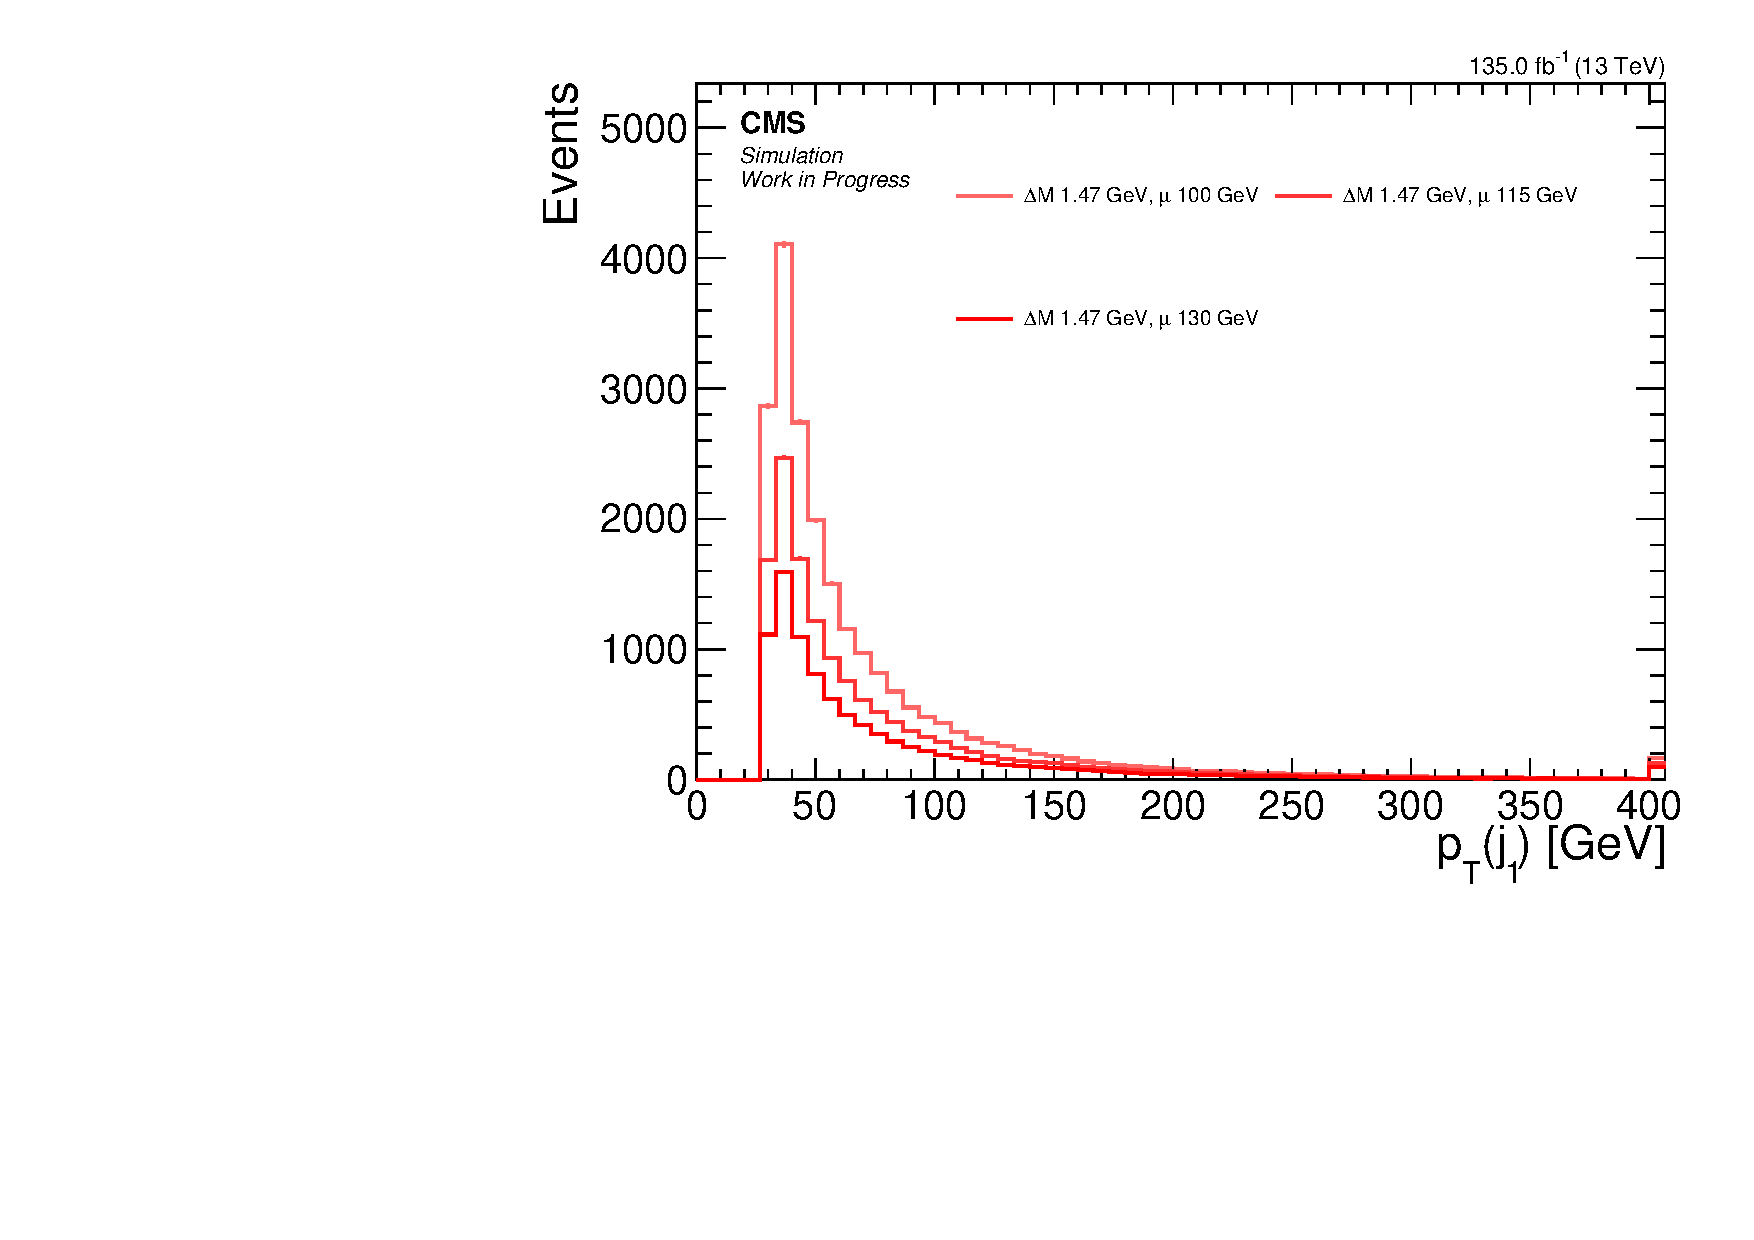
\includegraphics[width=0.48\linewidth]{plots/signal_common_distributions_fixed_dm/none_LeadingJetPt.pdf}  \\
\caption[Signal \emph{number of jets} and \emph{leading jet \pt} distributions]{ Signal distributions for \emph{number of jets} (left) and \emph{leading jet \pt} (right) comparing various $\dm$ with a fixed higgsino parameter $\mu=100\GeV$ (upper), and comparing various higgsino parameters $\mu$ with fixed $\dm=1.47\GeV$ (lower).}
\label{fig:signal-njets-ljpt}
\end{figure}

Our signal signature does not include a \PQb-jet, \ie, a jet resulting from a bottom quark hadronization (either resulting from a top quark or not). We therefore seek to exploit this knowledge by vetoing \PQb-tagged jets in the event. As described in \fxnote{add ref} we are using \DEEPCSV flavor tagging discriminant with a medium working point. As can be seen in these distributions, most of the signal lie in the 0 bin, and we will therefore veto any \PQb-tagged jet, which retains most of the signal, but rejects a lot of \gls{sm} background, such as arising from \ttbar events. 

\begin{figure}[h]
\centering
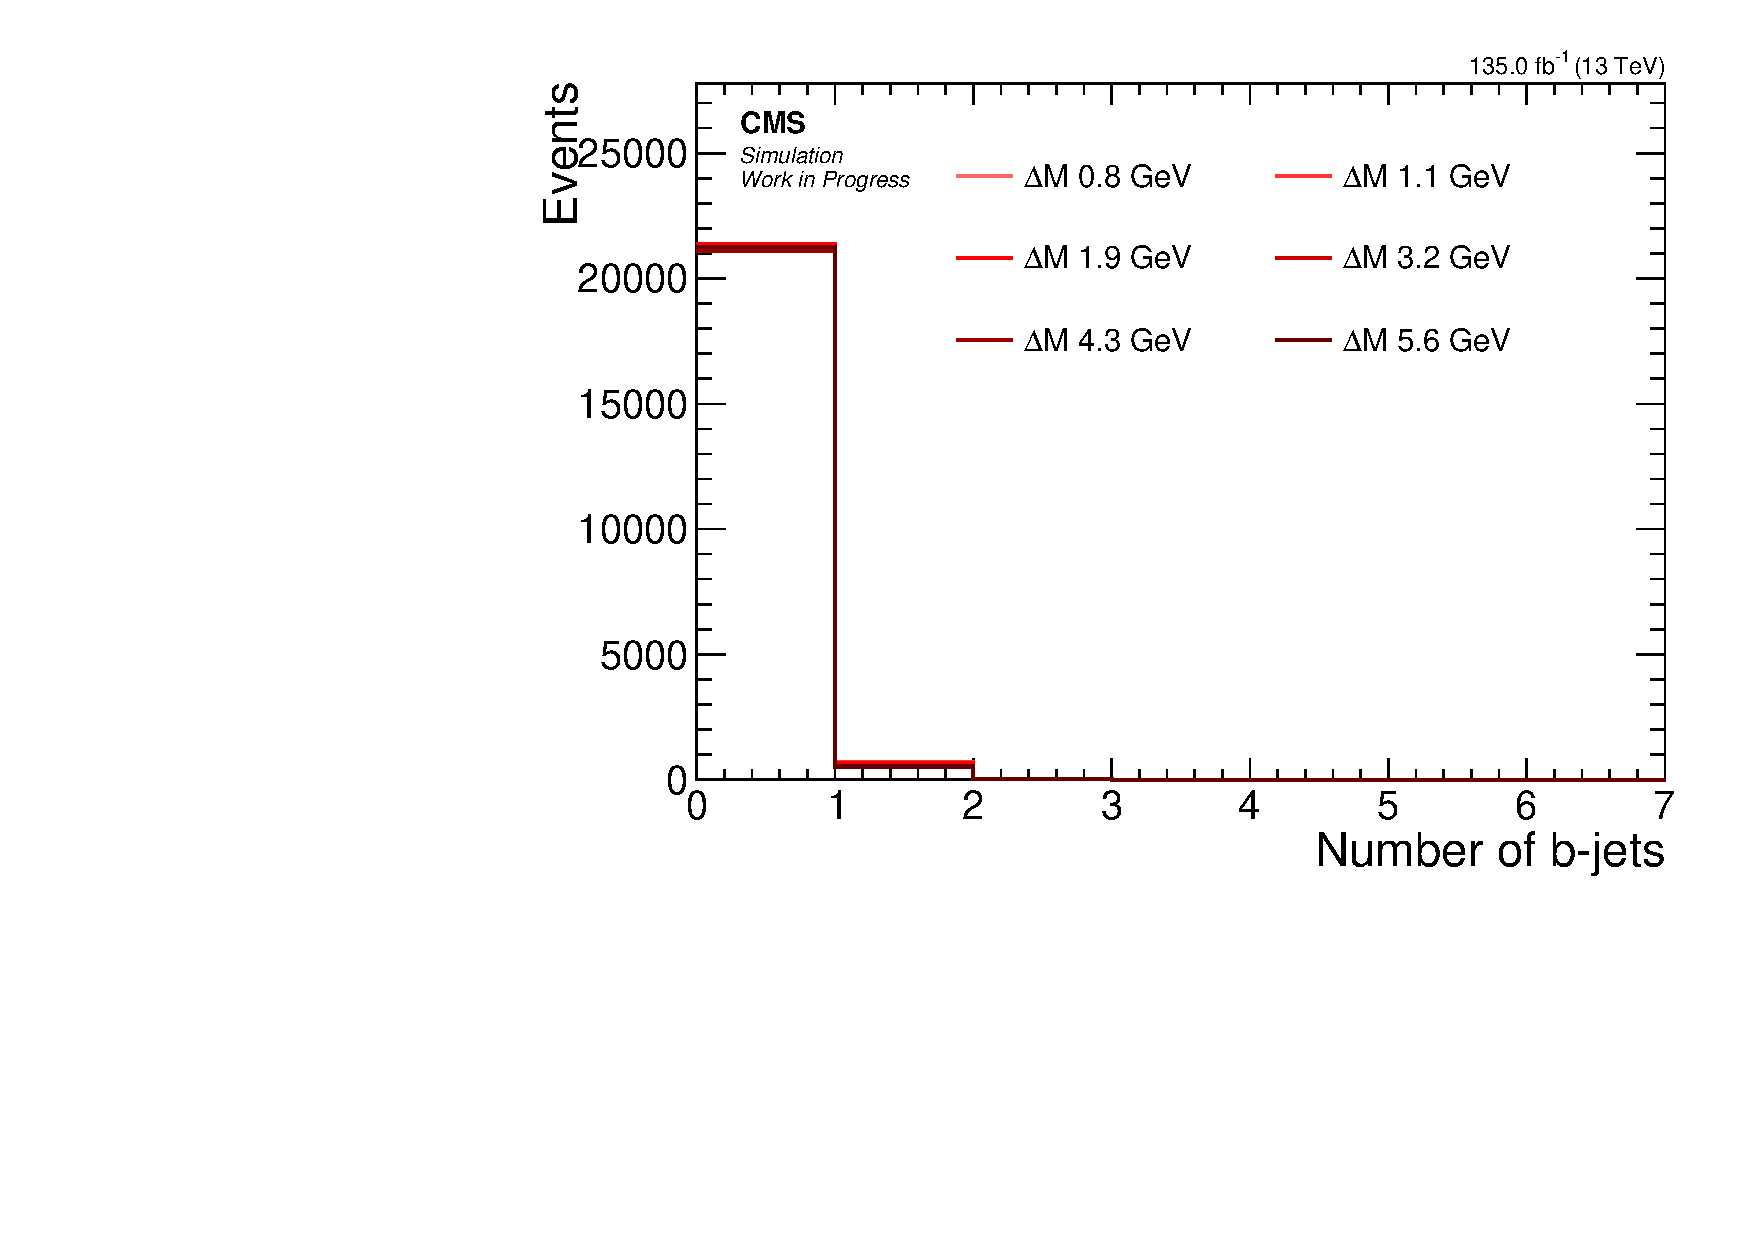
\includegraphics[width=0.48\linewidth]{plots/signal_common_distributions_fixed_mu/none_BTagsDeepMedium.pdf} \,
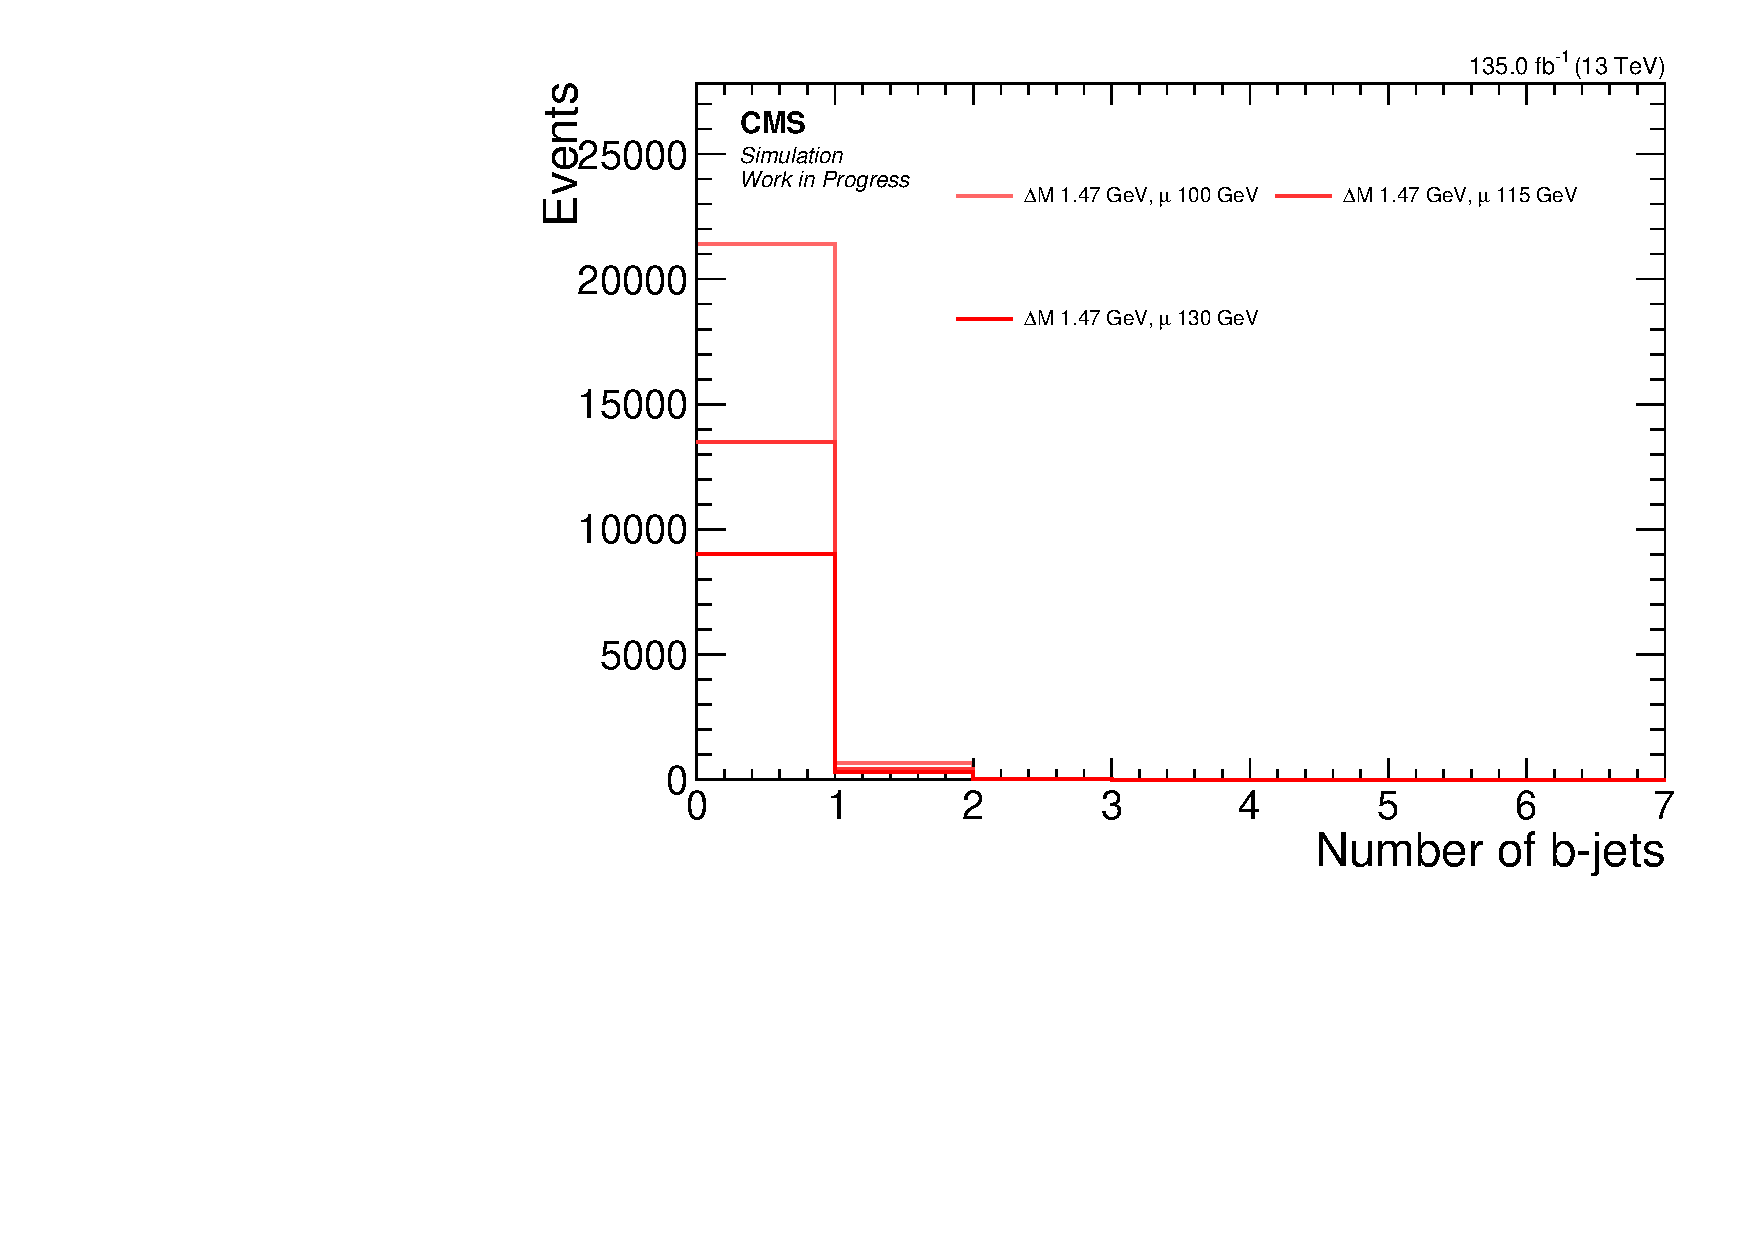
\includegraphics[width=0.48\linewidth]{plots/signal_common_distributions_fixed_dm/none_BTagsDeepMedium.pdf}  \\
\caption[Signal \emph{number of b-tagged jets} distributions]{ Signal distributions for \emph{number of b-tagged jets} comparing various $\dm$ with a fixed higgsino parameter $\mu=100\GeV$ (left), and comparing various higgsino parameters $\mu$ with fixed $\dm=1.47\GeV$ (right).}
\label{fig:signal-bjets}
\end{figure}

Since we are requiring an \gls{isr} jet in the event, we expect the \gls{met} and the \gls{mht} to point in the opposite direction of the jet, or at least in an angel close to $\pi$. Events with multiple jets in the \gls{sm} background such as arising from \gls{qcd} will not exhibit such a feature. In order to reduce \gls{qcd} background, we require $\mindphimhtjets > 0.4$.

\begin{figure}[h]
\centering
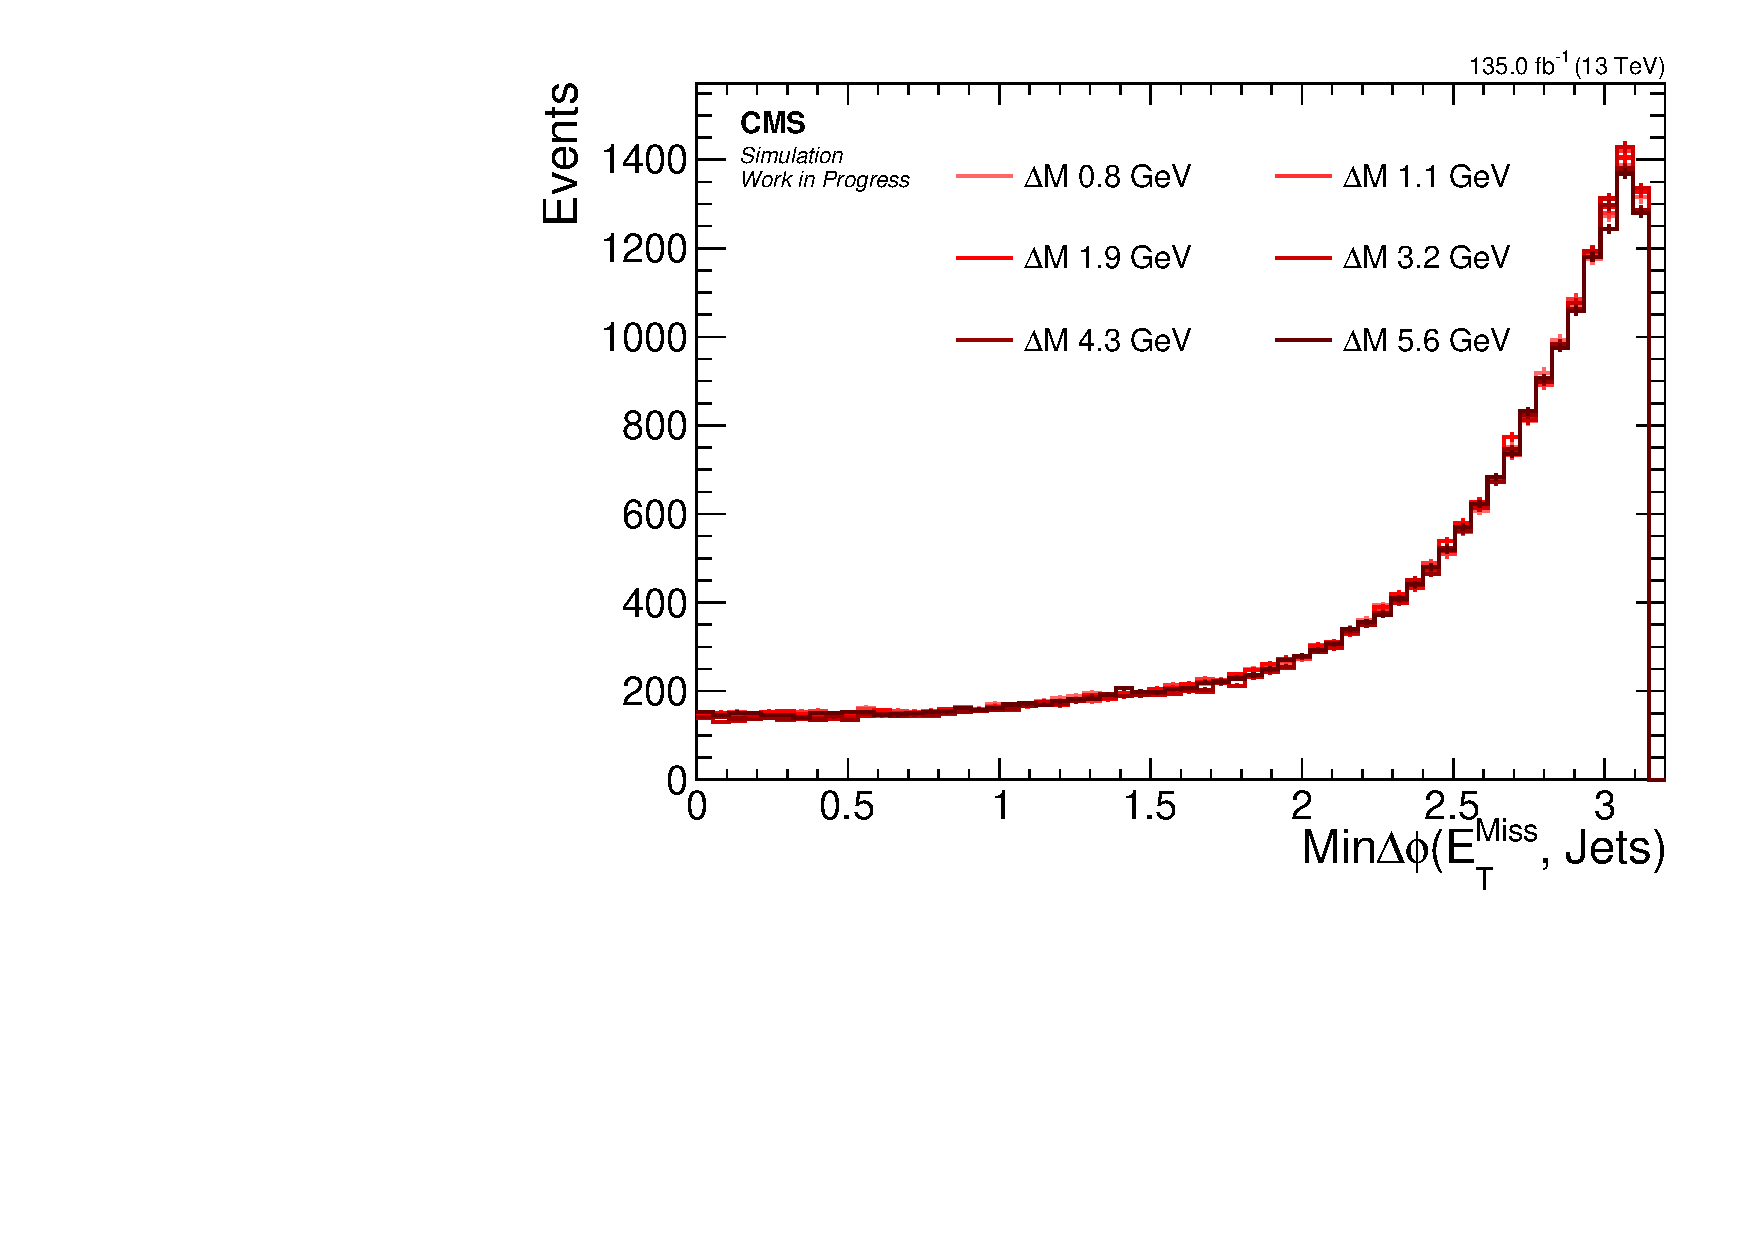
\includegraphics[width=0.48\linewidth]{plots/signal_common_distributions_fixed_mu/none_MinDeltaPhiMetJets.pdf} \,
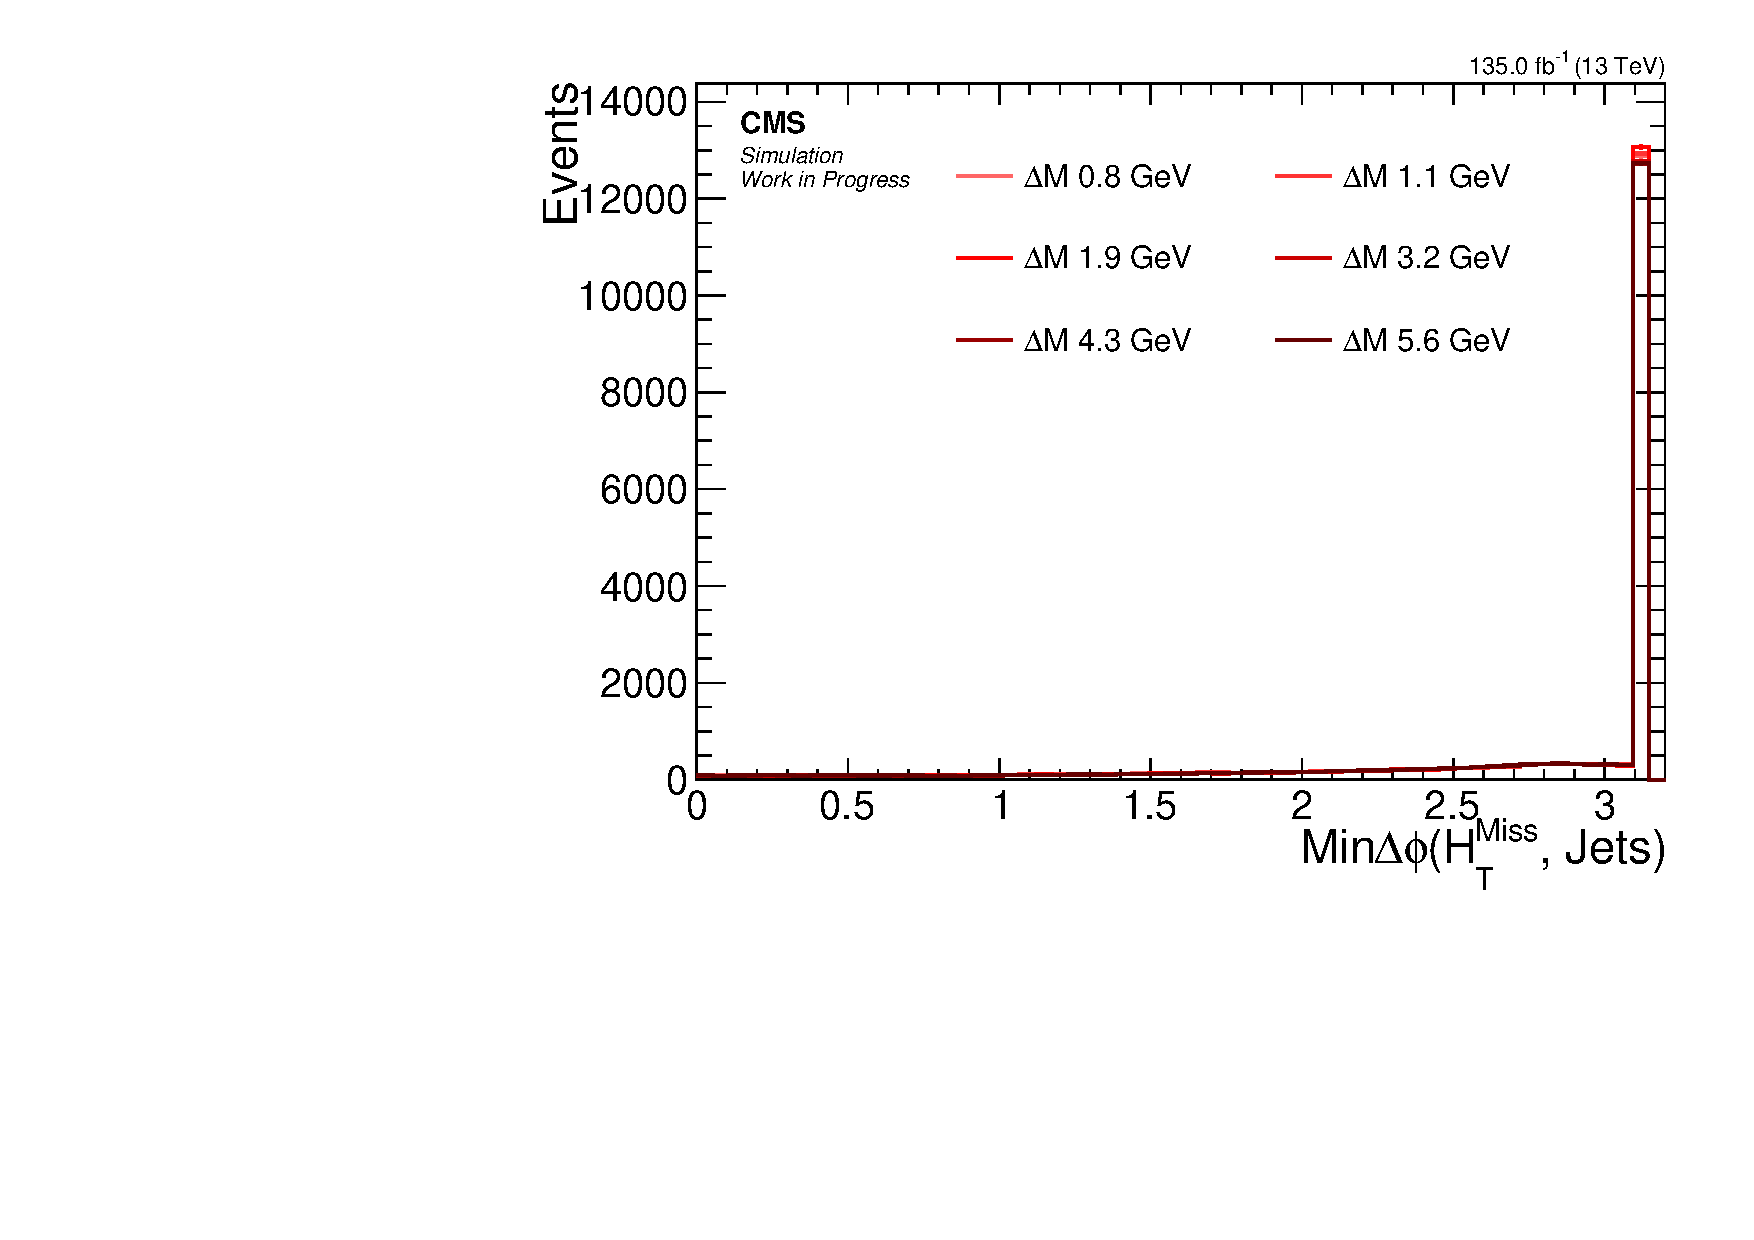
\includegraphics[width=0.48\linewidth]{plots/signal_common_distributions_fixed_mu/none_MinDeltaPhiMhtJets.pdf}  \\
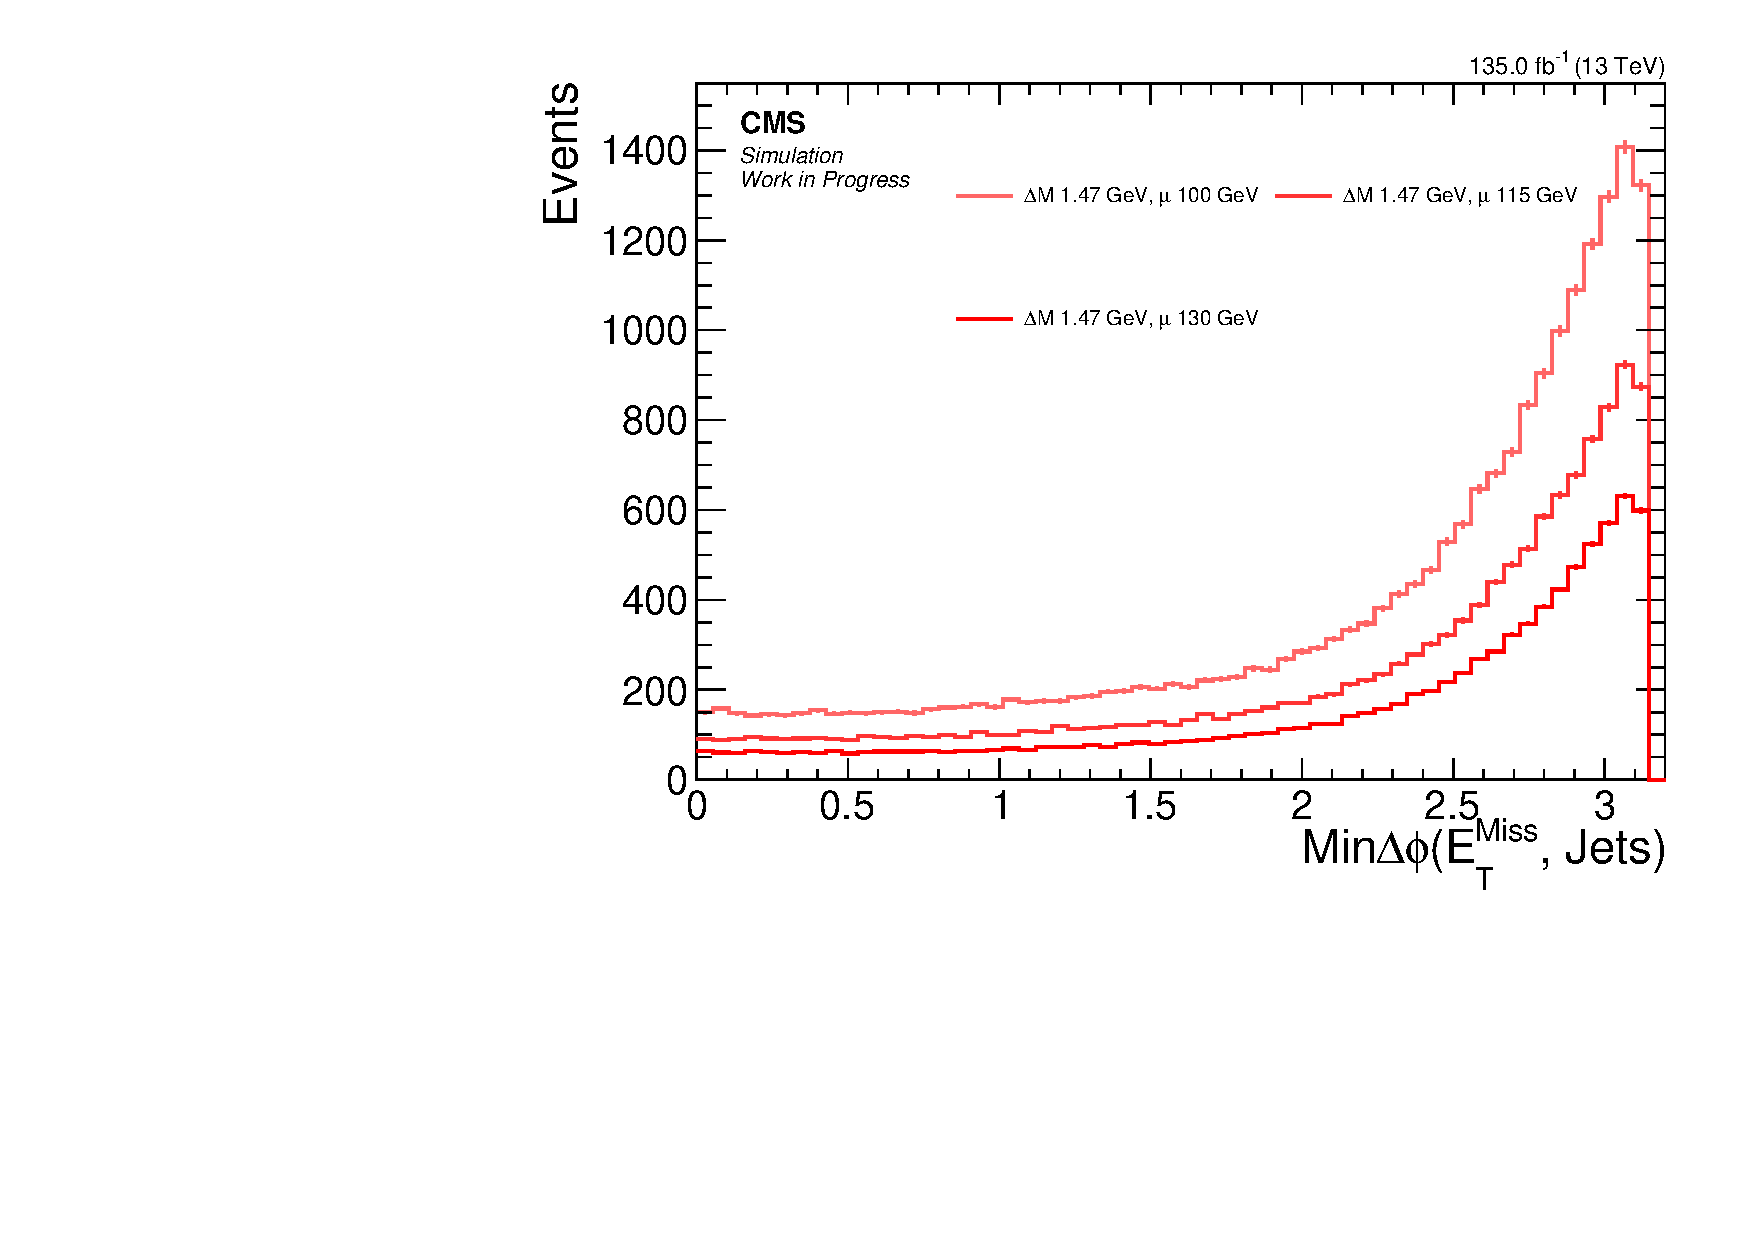
\includegraphics[width=0.48\linewidth]{plots/signal_common_distributions_fixed_dm/none_MinDeltaPhiMetJets.pdf} \,
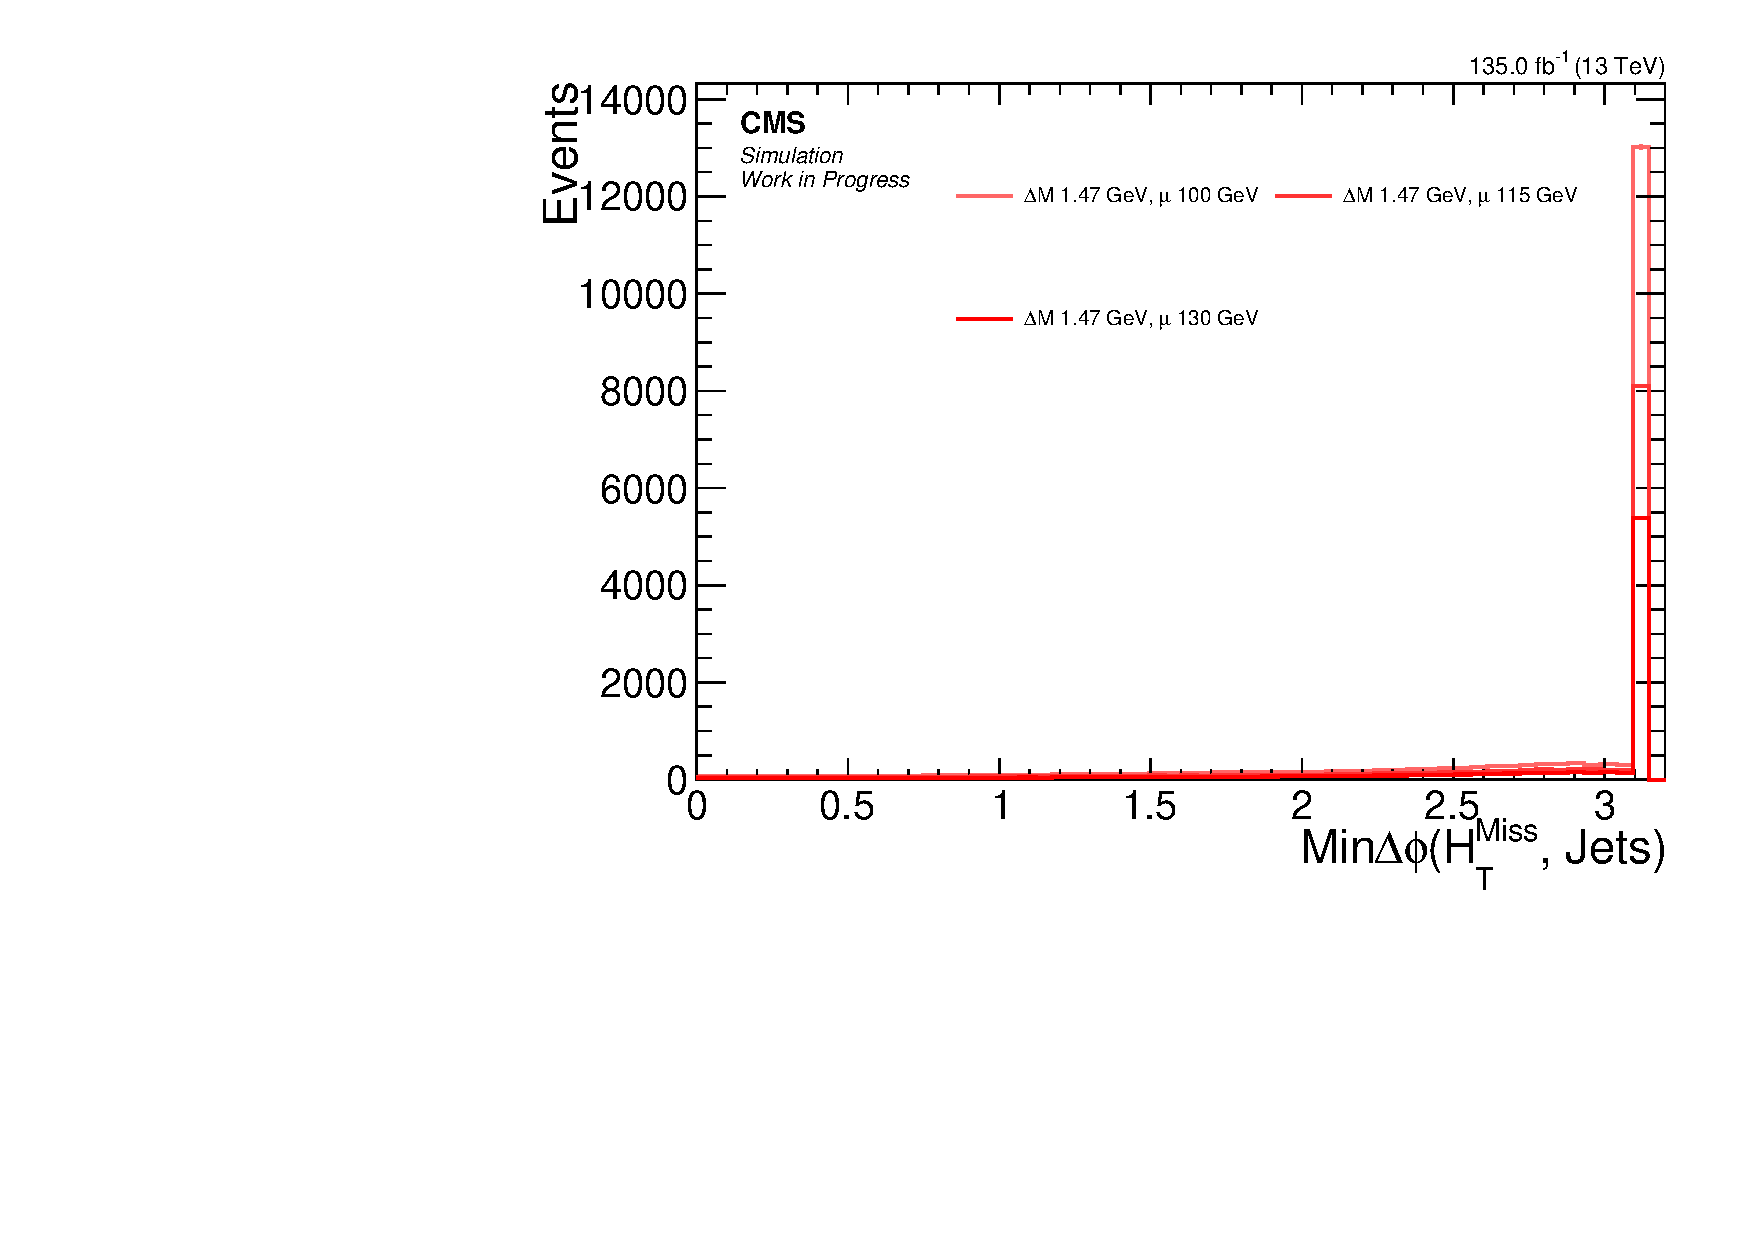
\includegraphics[width=0.48\linewidth]{plots/signal_common_distributions_fixed_dm/none_MinDeltaPhiMhtJets.pdf}  \\
\caption[Signal $\mindphimetjets$ and $\mindphimhtjets$ distributions]{ Signal distributions for \mindphimetjets (left) and \mindphimhtjets (right) comparing various $\dm$ with a fixed higgsino parameter $\mu=100\GeV$ (upper), and comparing various higgsino parameters $\mu$ with fixed $\dm=1.47\GeV$ (lower).}
\label{fig:signal-min-deltaphi-met-mht}
\end{figure}

\subsection{Base selection}

We recap the section by summarizing the base selection of our analysis. This base selection, or preselection as we might use call it interchangeably, is applied to all analysis categories. 

\begin{table}[hp]
	\centering
	\label{tab:base-selection}
		\caption{Base selection applied to all analysis categories}
		%\vspace{1mm}
			\begin{tabular}{lc} \hline
			Variable & Value \\ \hline
			$\mht \left[\GeV\right]$ & $\geq220$ \\
			$N_{\mathrm{jets}} \left( \pt \geq 30\GeV\, \mathrm{and}\, \abs{\eta} < 2.4 \right)$ & $\geq 1$\\
			$N_{\PQb-\mathrm{jets}} \left( \pt \geq 30\GeV\, \mathrm{and}\, \abs{\eta} < 2.4 \right)$ & 0 \\
			$\mindphimhtjets$ & $ > 0.4$ \\ \hline
			\end{tabular}
\end{table}